\documentclass{book}
\usepackage[T1]{fontenc}
\usepackage{babel}
\usepackage[dvipsnames,table]{xcolor}
\usepackage{ulem}
%https://mirrors.dotsrc.org/ctan/macros/luatex/latex/emoji/emoji-doc.pdf
\usepackage{emoji}
\usepackage[framemethod=tikz]{mdframed}
\usepackage{marginnote}
\setlength{\marginparwidth}{3cm}
\setlength{\marginparsep}{1cm}
\usepackage{amsmath,amsfonts,amssymb,amsthm}
\usepackage{booktabs}
\usepackage{multirow}
\usepackage{lilyglyphs} %https://www.ctan.org/pkg/lilyglyphs
\usepackage{array}
\usepackage{boldline}
\usepackage{etoolbox}
\usepackage[labelformat=empty]{caption}
\usepackage{wasysym}
\usepackage{fancyhdr}

\usepackage{csquotes}
\usepackage{animate}
\usepackage{hyperref}

\colorlet{cfemale}{RubineRed}
\colorlet{cmale}{BlueViolet}


\DeclareRobustCommand{\sovs}{
 \mbox{
  {\Large $\mathbb{S}_{O}$  }
  {\kern-1em\raise.8ex\hbox{V}\kern-.125em\@}
  {\kern-0.3em$\mathbb{S}$}
 }
}

\DeclareRobustCommand{\sovseneer}{
\mbox{
  {\Large $\mathbb{S}_{O}$  }
  {\kern-1em\raise.8ex\hbox{V}\kern-.125em\@}
  {\kern-0.3em$\mathbb{S}$}
  {\kern-0.3em\hbox{e}}
  {\kern-0.3em$\mathbb{N}$}
  {\Large $\sum_{}^{e}$ }
  {\kern-0.3em\hbox{R}}
 }
}

\DeclareRobustCommand{\sovsing}{
 \mbox{
  {\Large $\mathbb{S}_{O}$  }
  {\kern-1em\raise.8ex\hbox{V}\kern-.125em\@}
  {\kern-0.3em$\mathbb{S}_{\mathbb{I}ng}$}
 }
}

\mdfdefinestyle{scene}{
  leftmargin=-0.2cm,
  rightmargin=-2cm,
  roundcorner=10pt,
  frametitlerule=true,
  frametitlebackgroundcolor=gray!20
}


\mdtheorem[style=scene]{scene}{Scene}


%\kern-.36em%
%
 % {\sbox\z@ T%
%    \vbox to\ht\z@{\hbox{\check@mathfonts
 %   \fontsize\sf@size\z@  
%    \math@fontsfalse\selectfont
%    A}%
%  \vss}%
%}%
%\kern-.15em%
%\TeX}

\author{Sunetiago Hansen}
\title{Simrebogen}

\begin{document}
\pagestyle{fancy}
\fancyhead{}
\fancyhead[RO,LE]{Simrebogen - The \sovs manifesto}

\newcommand{\scactorf}[1]{{\color{cfemale}\textbf{\textit{#1}}}}
\newcommand{\scactorm}[1]{{\color{cmale}\textbf{\textit{#1}}}}
\newcommand{\sovsatt}[1]{{\textit{#1}}}




%----------------------------------------------------------------------------------------
%	TITLE PAGE
%----------------------------------------------------------------------------------------

\begin{titlepage} % Suppresses headers and footers on the title page

	\raggedleft % Right align everything
	
	\vspace*{\baselineskip} % Whitespace at the top of the page
	
	%------------------------------------------------
	%	Author
	%------------------------------------------------
	
	{\Large Sunetiago Hansen} % Author name
	
	\vspace*{0.167\textheight} % Whitespace before the title
	
	%------------------------------------------------
	%	Title and subtitle
	%------------------------------------------------
	
	%\textbf{\LARGE The Big Book of}\\[\baselineskip] % First title line
	
	{\textcolor{Gray}{\Huge Simrebogen v. 1.0}}\\[\baselineskip] % Main title line which draws the focus of the reader
	
	{\Large\textit{The \sovs manifesto}} % Subtitle
	
	\vfill % Whitespace between the titles and the publisher
	\begin{center}
           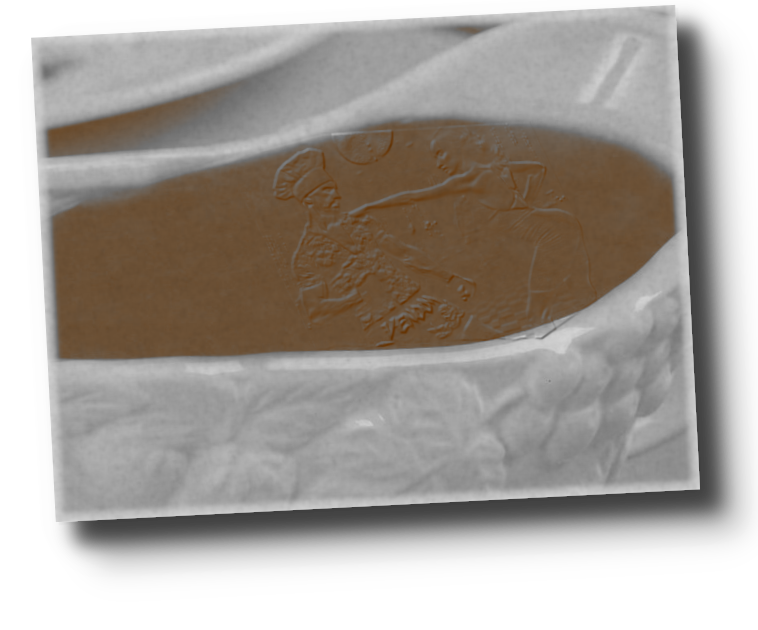
\includegraphics[scale=2.2]{Frontpage/sovs-front-page}
	\end{center}

	%------------------------------------------------
	%	Publisher
	%------------------------------------------------
	
	%{\large ~~\plogo} % Publisher and logo
	
	\vspace*{3\baselineskip} % Whitespace at the bottom of the page

\end{titlepage}

\pagebreak{}
\begin{center}
{\Large
\textit{\textbf{The story of \sovs}}
}
\\
\vspace{0.5cm}
\textbf{Part I} -\textit{ The \textbf{epidemic} stage}
\end{center}

%\part{Foundations of Sovs}
%\input{00-principles/principles.tex}





\newpage
\end{document}